%%%%%%%%%%%%%%%%%%%%%%%%%%%%%%%%%%%%%%%%%
% The Legrand Orange Book
% LaTeX Template
% Version 2.3 (8/8/17)
%
% This template has been downloaded from:
% http://www.LaTeXTemplates.com
%
% Original author:
% Mathias Legrand (legrand.mathias@gmail.com) with modifications by:
% Vel (vel@latextemplates.com)
%
% License:
% CC BY-NC-SA 3.0 (http://creativecommons.org/licenses/by-nc-sa/3.0/)
%
% Compiling this template:
% This template uses biber for its bibliography and makeindex for its index.
% When you first open the template, compile it from the command line with the 
% commands below to make sure your LaTeX distribution is configured correctly:
%
% 1) pdflatex main
% 2) makeindex main.idx -s StyleInd.ist
% 3) biber main
% 4) pdflatex main x 2
%
% After this, when you wish to update the bibliography/index use the appropriate
% command above and make sure to compile with pdflatex several times 
% afterwards to propagate your changes to the document.
%
% This template also uses a number of packages which may need to be
% updated to the newest versions for the template to compile. It is strongly
% recommended you update your LaTeX distribution if you have any
% compilation errors.
%
% Important note:
% Chapter heading images should have a 2:1 width:height ratio,
% e.g. 920px width and 460px height.
%
%%%%%%%%%%%%%%%%%%%%%%%%%%%%%%%%%%%%%%%%%

%----------------------------------------------------------------------------------------
%	PACKAGES AND OTHER DOCUMENT CONFIGURATIONS
%----------------------------------------------------------------------------------------

\documentclass[12pt,fleqn,openany]{book} % Default font size and left-justified equations
\usepackage{wrapfig}
\usepackage{algorithm2e}
%----------------------------------------------------------------------------------------

%%%%%%%%%%%%%%%%%%%%%%%%%%%%%%%%%%%%%%%%%
% The Legrand Orange Book
% Structural Definitions File
% Version 2.0 (9/2/15)
%
% Original author:
% Mathias Legrand (legrand.mathias@gmail.com) with modifications by:
% Vel (vel@latextemplates.com)
% 
% This file has been downloaded from:
% http://www.LaTeXTemplates.com
%
% License:
% CC BY-NC-SA 3.0 (http://creativecommons.org/licenses/by-nc-sa/3.0/)
%
%%%%%%%%%%%%%%%%%%%%%%%%%%%%%%%%%%%%%%%%%

%----------------------------------------------------------------------------------------
%	VARIOUS REQUIRED PACKAGES AND CONFIGURATIONS
%----------------------------------------------------------------------------------------

\usepackage[top=3cm,bottom=3cm,left=3cm,right=3cm,headsep=10pt,a4paper]{geometry} % Page margins

\usepackage{graphicx} % Required for including pictures
\graphicspath{{Pictures/}} % Specifies the directory where pictures are stored

\usepackage{lipsum} % Inserts dummy text

\usepackage{tikz} % Required for drawing custom shapes

\usepackage[swedish]{babel} % English language/hyphenation

\usepackage{enumitem} % Customize lists
\setlist{nolistsep} % Reduce spacing between bullet points and numbered lists

\usepackage{booktabs} % Required for nicer horizontal rules in tables

\usepackage{xcolor} % Required for specifying colors by name
\definecolor{ocre}{RGB}{243,102,25} % Define the orange color used for highlighting throughout the book

%----------------------------------------------------------------------------------------
%	FONTS
%----------------------------------------------------------------------------------------

\usepackage{avant} % Use the Avantgarde font for headings
%\usepackage{times} % Use the Times font for headings
\usepackage{mathptmx} % Use the Adobe Times Roman as the default text font together with math symbols from the Sym­bol, Chancery and Com­puter Modern fonts

\usepackage{microtype} % Slightly tweak font spacing for aesthetics
\usepackage[utf8]{inputenc} % Required for including letters with accents
\usepackage[T1]{fontenc} % Use 8-bit encoding that has 256 glyphs

%----------------------------------------------------------------------------------------
%	BIBLIOGRAPHY AND INDEX
%----------------------------------------------------------------------------------------

\usepackage[style=numeric,citestyle=numeric,sorting=nyt,sortcites=true,autopunct=true,babel=hyphen,hyperref=true,abbreviate=false,backref=true,backend=biber]{biblatex}
\addbibresource{bibliography.bib} % BibTeX bibliography file
\defbibheading{bibempty}{}

\usepackage{calc} % For simpler calculation - used for spacing the index letter headings correctly
\usepackage{makeidx} % Required to make an index
\makeindex % Tells LaTeX to create the files required for indexing

%----------------------------------------------------------------------------------------
%	MAIN TABLE OF CONTENTS
%----------------------------------------------------------------------------------------

\usepackage{titletoc} % Required for manipulating the table of contents

\contentsmargin{0cm} % Removes the default margin

% Part text styling
\titlecontents{part}[0cm]
{\addvspace{20pt}\centering\large\bfseries}
{}
{}
{}

% Chapter text styling
\titlecontents{chapter}[1.25cm] % Indentation
{\addvspace{12pt}\large\sffamily\bfseries} % Spacing and font options for chapters
{\color{ocre!60}\contentslabel[\Large\thecontentslabel]{1.25cm}\color{ocre}} % Chapter number
{\color{ocre}}  
{\color{ocre!60}\normalsize\;\titlerule*[.5pc]{.}\;\thecontentspage} % Page number

% Section text styling
\titlecontents{section}[1.25cm] % Indentation
{\addvspace{3pt}\sffamily\bfseries} % Spacing and font options for sections
{\contentslabel[\thecontentslabel]{1.25cm}} % Section number
{}
{\hfill\color{black}\thecontentspage} % Page number
[]

% Subsection text styling
\titlecontents{subsection}[1.25cm] % Indentation
{\addvspace{1pt}\sffamily\small} % Spacing and font options for subsections
{\contentslabel[\thecontentslabel]{1.25cm}} % Subsection number
{}
{\ \titlerule*[.5pc]{.}\;\thecontentspage} % Page number
[]

% List of figures
\titlecontents{figure}[0em]
{\addvspace{-5pt}\sffamily}
{\thecontentslabel\hspace*{1em}}
{}
{\ \titlerule*[.5pc]{.}\;\thecontentspage}
[]

% List of tables
\titlecontents{table}[0em]
{\addvspace{-5pt}\sffamily}
{\thecontentslabel\hspace*{1em}}
{}
{\ \titlerule*[.5pc]{.}\;\thecontentspage}
[]

%----------------------------------------------------------------------------------------
%	MINI TABLE OF CONTENTS IN PART HEADS
%----------------------------------------------------------------------------------------

% Chapter text styling
\titlecontents{lchapter}[0em] % Indenting
{\addvspace{15pt}\large\sffamily\bfseries} % Spacing and font options for chapters
{\color{ocre}\contentslabel[\Large\thecontentslabel]{1.25cm}\color{ocre}} % Chapter number
{}  
{\color{ocre}\normalsize\sffamily\bfseries\;\titlerule*[.5pc]{.}\;\thecontentspage} % Page number

% Section text styling
\titlecontents{lsection}[0em] % Indenting
{\sffamily\small} % Spacing and font options for sections
{\contentslabel[\thecontentslabel]{1.25cm}} % Section number
{}
{}

% Subsection text styling
\titlecontents{lsubsection}[.5em] % Indentation
{\normalfont\footnotesize\sffamily} % Font settings
{}
{}
{}

%----------------------------------------------------------------------------------------
%	PAGE HEADERS
%----------------------------------------------------------------------------------------

\usepackage{fancyhdr} % Required for header and footer configuration

\pagestyle{fancy}
\renewcommand{\chaptermark}[1]{\markboth{\sffamily\normalsize\bfseries\chaptername\ \thechapter.\ #1}{}} % Chapter text font settings
\renewcommand{\sectionmark}[1]{\markright{\sffamily\normalsize\thesection\hspace{5pt}#1}{}} % Section text font settings
\fancyhf{} \fancyhead[LE,RO]{\sffamily\normalsize\thepage} % Font setting for the page number in the header
\fancyhead[LO]{\rightmark} % Print the nearest section name on the left side of odd pages
\fancyhead[RE]{\leftmark} % Print the current chapter name on the right side of even pages
\renewcommand{\headrulewidth}{0.5pt} % Width of the rule under the header
\addtolength{\headheight}{2.5pt} % Increase the spacing around the header slightly
\renewcommand{\footrulewidth}{0pt} % Removes the rule in the footer
\fancypagestyle{plain}{\fancyhead{}\renewcommand{\headrulewidth}{0pt}} % Style for when a plain pagestyle is specified

% Removes the header from odd empty pages at the end of chapters
\makeatletter
\renewcommand{\cleardoublepage}{
\clearpage\ifodd\c@page\else
\hbox{}
\vspace*{\fill}
\thispagestyle{empty}
\newpage
\fi}

%----------------------------------------------------------------------------------------
%	THEOREM STYLES
%----------------------------------------------------------------------------------------

\usepackage{amsmath,amsfonts,amssymb,amsthm} % For math equations, theorems, symbols, etc

\newcommand{\intoo}[2]{\mathopen{]}#1\,;#2\mathclose{[}}
\newcommand{\ud}{\mathop{\mathrm{{}d}}\mathopen{}}
\newcommand{\intff}[2]{\mathopen{[}#1\,;#2\mathclose{]}}
\newtheorem{notation}{Notation}[chapter]

% Boxed/framed environments
\newtheoremstyle{ocrenumbox}% % Theorem style name
{0pt}% Space above
{0pt}% Space below
{\normalfont}% % Body font
{}% Indent amount
{\small\bf\sffamily\color{ocre}}% % Theorem head font
{\;}% Punctuation after theorem head
{0.25em}% Space after theorem head
{\small\sffamily\color{ocre}\thmname{#1}\nobreakspace\thmnumber{\@ifnotempty{#1}{}\@upn{#2}}% Theorem text (e.g. Theorem 2.1)
\thmnote{\nobreakspace\the\thm@notefont\sffamily\bfseries\color{black}---\nobreakspace#3.}} % Optional theorem note
\renewcommand{\qedsymbol}{$\blacksquare$}% Optional qed square

\newtheoremstyle{blacknumex}% Theorem style name
{5pt}% Space above
{5pt}% Space below
{\normalfont}% Body font
{} % Indent amount
{\small\bf\sffamily}% Theorem head font
{\;}% Punctuation after theorem head
{0.25em}% Space after theorem head
{\small\sffamily{\tiny\ensuremath{\blacksquare}}\nobreakspace\thmname{#1}\nobreakspace\thmnumber{\@ifnotempty{#1}{}\@upn{#2}}% Theorem text (e.g. Theorem 2.1)
\thmnote{\nobreakspace\the\thm@notefont\sffamily\bfseries---\nobreakspace#3.}}% Optional theorem note

\newtheoremstyle{blacknumbox} % Theorem style name
{0pt}% Space above
{0pt}% Space below
{\normalfont}% Body font
{}% Indent amount
{\small\bf\sffamily}% Theorem head font
{\;}% Punctuation after theorem head
{0.25em}% Space after theorem head
{\small\sffamily\thmname{#1}\nobreakspace\thmnumber{\@ifnotempty{#1}{}\@upn{#2}}% Theorem text (e.g. Theorem 2.1)
\thmnote{\nobreakspace\the\thm@notefont\sffamily\bfseries---\nobreakspace#3.}}% Optional theorem note

% Non-boxed/non-framed environments
\newtheoremstyle{ocrenum}% % Theorem style name
{5pt}% Space above
{5pt}% Space below
{\normalfont}% % Body font
{}% Indent amount
{\small\bf\sffamily\color{ocre}}% % Theorem head font
{\;}% Punctuation after theorem head
{0.25em}% Space after theorem head
{\small\sffamily\color{ocre}\thmname{#1}\nobreakspace\thmnumber{\@ifnotempty{#1}{}\@upn{#2}}% Theorem text (e.g. Theorem 2.1)
\thmnote{\nobreakspace\the\thm@notefont\sffamily\bfseries\color{black}---\nobreakspace#3.}} % Optional theorem note
\renewcommand{\qedsymbol}{$\blacksquare$}% Optional qed square
\makeatother

% Defines the theorem text style for each type of theorem to one of the three styles above
\newcounter{dummy} 
\numberwithin{dummy}{section}
\theoremstyle{ocrenumbox}
\newtheorem{theoremeT}[dummy]{Theorem}
\newtheorem{problem}{Problem}[chapter]
\newtheorem{exerciseT}{Exercise}[chapter]
\theoremstyle{blacknumex}
\newtheorem{exampleT}{Example}[chapter]
\theoremstyle{blacknumbox}
\newtheorem{vocabulary}{Vocabulary}[chapter]
\newtheorem{definitionT}{Definition}[section]
\newtheorem{corollaryT}[dummy]{Corollary}
\theoremstyle{ocrenum}
\newtheorem{proposition}[dummy]{Proposition}

%----------------------------------------------------------------------------------------
%	DEFINITION OF COLORED BOXES
%----------------------------------------------------------------------------------------

\RequirePackage[framemethod=default]{mdframed} % Required for creating the theorem, definition, exercise and corollary boxes

% Theorem box
\newmdenv[skipabove=7pt,
skipbelow=7pt,
backgroundcolor=black!5,
linecolor=ocre,
innerleftmargin=5pt,
innerrightmargin=5pt,
innertopmargin=5pt,
leftmargin=0cm,
rightmargin=0cm,
innerbottommargin=5pt]{tBox}

% Exercise box	  
\newmdenv[skipabove=7pt,
skipbelow=7pt,
rightline=false,
leftline=true,
topline=false,
bottomline=false,
backgroundcolor=ocre!10,
linecolor=ocre,
innerleftmargin=5pt,
innerrightmargin=5pt,
innertopmargin=5pt,
innerbottommargin=5pt,
leftmargin=0cm,
rightmargin=0cm,
linewidth=4pt]{eBox}	

% Definition box
\newmdenv[skipabove=7pt,
skipbelow=7pt,
rightline=false,
leftline=true,
topline=false,
bottomline=false,
linecolor=ocre,
innerleftmargin=5pt,
innerrightmargin=5pt,
innertopmargin=0pt,
leftmargin=0cm,
rightmargin=0cm,
linewidth=4pt,
innerbottommargin=0pt]{dBox}	

% Corollary box
\newmdenv[skipabove=7pt,
skipbelow=7pt,
rightline=false,
leftline=true,
topline=false,
bottomline=false,
linecolor=gray,
backgroundcolor=black!5,
innerleftmargin=5pt,
innerrightmargin=5pt,
innertopmargin=5pt,
leftmargin=0cm,
rightmargin=0cm,
linewidth=4pt,
innerbottommargin=5pt]{cBox}

% Creates an environment for each type of theorem and assigns it a theorem text style from the "Theorem Styles" section above and a colored box from above
\newenvironment{theorem}{\begin{tBox}\begin{theoremeT}}{\end{theoremeT}\end{tBox}}
\newenvironment{exercise}{\begin{eBox}\begin{exerciseT}}{\hfill{\color{ocre}\tiny\ensuremath{\blacksquare}}\end{exerciseT}\end{eBox}}				  
\newenvironment{definition}{\begin{dBox}\begin{definitionT}}{\end{definitionT}\end{dBox}}	
\newenvironment{example}{\begin{exampleT}}{\hfill{\tiny\ensuremath{\blacksquare}}\end{exampleT}}		
\newenvironment{corollary}{\begin{cBox}\begin{corollaryT}}{\end{corollaryT}\end{cBox}}	

%----------------------------------------------------------------------------------------
%	REMARK ENVIRONMENT
%----------------------------------------------------------------------------------------

\newenvironment{remark}{\par\vspace{10pt}\small % Vertical white space above the remark and smaller font size
\begin{list}{}{
\leftmargin=35pt % Indentation on the left
\rightmargin=25pt}\item\ignorespaces % Indentation on the right
\makebox[-2.5pt]{\begin{tikzpicture}[overlay]
\node[draw=ocre!60,line width=1pt,circle,fill=ocre!25,font=\sffamily\bfseries,inner sep=2pt,outer sep=0pt] at (-15pt,0pt){\textcolor{ocre}{R}};\end{tikzpicture}} % Orange R in a circle
\advance\baselineskip -1pt}{\end{list}\vskip5pt} % Tighter line spacing and white space after remark

%----------------------------------------------------------------------------------------
%	SECTION NUMBERING IN THE MARGIN
%----------------------------------------------------------------------------------------

\makeatletter
\renewcommand{\@seccntformat}[1]{\llap{\textcolor{ocre}{\csname the#1\endcsname}\hspace{1em}}}                    
\renewcommand{\section}{\@startsection{section}{1}{\z@}
{-4ex \@plus -1ex \@minus -.4ex}
{1ex \@plus.2ex }
{\normalfont\large\sffamily\bfseries}}
\renewcommand{\subsection}{\@startsection {subsection}{2}{\z@}
{-3ex \@plus -0.1ex \@minus -.4ex}
{0.5ex \@plus.2ex }
{\normalfont\sffamily\bfseries}}
\renewcommand{\subsubsection}{\@startsection {subsubsection}{3}{\z@}
{-2ex \@plus -0.1ex \@minus -.2ex}
{.2ex \@plus.2ex }
{\normalfont\small\sffamily\bfseries}}                        
\renewcommand\paragraph{\@startsection{paragraph}{4}{\z@}
{-2ex \@plus-.2ex \@minus .2ex}
{.1ex}
{\normalfont\small\sffamily\bfseries}}

%----------------------------------------------------------------------------------------
%	PART HEADINGS
%----------------------------------------------------------------------------------------

% numbered part in the table of contents
\newcommand{\@mypartnumtocformat}[2]{%
\setlength\fboxsep{0pt}%
\noindent\colorbox{ocre!20}{\strut\parbox[c][.7cm]{\ecart}{\color{ocre!70}\Large\sffamily\bfseries\centering#1}}\hskip\esp\colorbox{ocre!40}{\strut\parbox[c][.7cm]{\linewidth-\ecart-\esp}{\Large\sffamily\centering#2}}}%
%%%%%%%%%%%%%%%%%%%%%%%%%%%%%%%%%%
% unnumbered part in the table of contents
\newcommand{\@myparttocformat}[1]{%
\setlength\fboxsep{0pt}%
\noindent\colorbox{ocre!40}{\strut\parbox[c][.7cm]{\linewidth}{\Large\sffamily\centering#1}}}%
%%%%%%%%%%%%%%%%%%%%%%%%%%%%%%%%%%
\newlength\esp
\setlength\esp{4pt}
\newlength\ecart
\setlength\ecart{1.2cm-\esp}
\newcommand{\thepartimage}{}%
\newcommand{\partimage}[1]{\renewcommand{\thepartimage}{#1}}%
\def\@part[#1]#2{%
\ifnum \c@secnumdepth >-2\relax%
\refstepcounter{part}%
\addcontentsline{toc}{part}{\texorpdfstring{\protect\@mypartnumtocformat{\thepart}{#1}}{\partname~\thepart\ ---\ #1}}
\else%
\addcontentsline{toc}{part}{\texorpdfstring{\protect\@myparttocformat{#1}}{#1}}%
\fi%
\startcontents%
\markboth{}{}%
{\thispagestyle{empty}%
\begin{tikzpicture}[remember picture,overlay]%
\node at (current page.north west){\begin{tikzpicture}[remember picture,overlay]%	
\fill[ocre!20](0cm,0cm) rectangle (\paperwidth,-\paperheight);
\node[anchor=north] at (4cm,-3.25cm){\color{ocre!40}\fontsize{220}{100}\sffamily\bfseries\thepart}; 
\node[anchor=south east] at (\paperwidth-1cm,-\paperheight+1cm){\parbox[t][][t]{8.5cm}{
\printcontents{l}{0}{\setcounter{tocdepth}{1}}%
}};
\node[anchor=north east] at (\paperwidth-1.5cm,-3.25cm){\parbox[t][][t]{15cm}{\strut\raggedleft\color{white}\fontsize{30}{30}\sffamily\bfseries#2}};
\end{tikzpicture}};
\end{tikzpicture}}%
\@endpart}
\def\@spart#1{%
\startcontents%
\phantomsection
{\thispagestyle{empty}%
\begin{tikzpicture}[remember picture,overlay]%
\node at (current page.north west){\begin{tikzpicture}[remember picture,overlay]%	
\fill[ocre!20](0cm,0cm) rectangle (\paperwidth,-\paperheight);
\node[anchor=north east] at (\paperwidth-1.5cm,-3.25cm){\parbox[t][][t]{15cm}{\strut\raggedleft\color{white}\fontsize{30}{30}\sffamily\bfseries#1}};
\end{tikzpicture}};
\end{tikzpicture}}
\addcontentsline{toc}{part}{\texorpdfstring{%
\setlength\fboxsep{0pt}%
\noindent\protect\colorbox{ocre!40}{\strut\protect\parbox[c][.7cm]{\linewidth}{\Large\sffamily\protect\centering #1\quad\mbox{}}}}{#1}}%
\@endpart}
\def\@endpart{\vfil\newpage
\if@twoside
\if@openright
\null
\thispagestyle{empty}%
\newpage
\fi
\fi
\if@tempswa
\twocolumn
\fi}

%----------------------------------------------------------------------------------------
%	CHAPTER HEADINGS
%----------------------------------------------------------------------------------------

% A switch to conditionally include a picture, implemented by  Christian Hupfer
\newif\ifusechapterimage
\usechapterimagetrue
\newcommand{\thechapterimage}{}%
\newcommand{\chapterimage}[1]{\ifusechapterimage\renewcommand{\thechapterimage}{#1}\fi}%
\newcommand{\autodot}{.}
\def\@makechapterhead#1{%
{\parindent \z@ \raggedright \normalfont
\ifnum \c@secnumdepth >\m@ne
\if@mainmatter
\begin{tikzpicture}[remember picture,overlay]
\node at (current page.north west)
{\begin{tikzpicture}[remember picture,overlay]
\node[anchor=north west,inner sep=0pt] at (0,0) {\ifusechapterimage\includegraphics[width=\paperwidth]{\thechapterimage}\fi};
\draw[anchor=west] (\Gm@lmargin,-9.7cm) node [line width=2pt,rounded corners=15pt,draw=ocre,fill=black,fill opacity=0.5,inner sep=9pt]{\strut\makebox[22cm]{}};
\draw[anchor=west] (\Gm@lmargin+.3cm,-9.8cm) node {\huge\sffamily\bfseries\color{white}\thechapter\autodot~#1\strut};
\end{tikzpicture}};
\end{tikzpicture}
\else
\begin{tikzpicture}[remember picture,overlay]
\node at (current page.north west)
{\begin{tikzpicture}[remember picture,overlay]
\node[anchor=north west,inner sep=0pt] at (0,0) {\ifusechapterimage\includegraphics[width=\paperwidth]{\thechapterimage}\fi};
\draw[anchor=west] (\Gm@lmargin,-9.7cm) node [line width=2pt,rounded corners=15pt,draw=ocre,fill=black,fill opacity=0.5,inner sep=9pt]{\strut\makebox[22cm]{}};
\draw[anchor=west] (\Gm@lmargin+.3cm,-9.8cm) node {\huge\sffamily\bfseries\color{white}#1\strut};
\end{tikzpicture}};
\end{tikzpicture}
\fi\fi\par\vspace*{270\p@}}}

%-------------------------------------------

\def\@makeschapterhead#1{%
\begin{tikzpicture}[remember picture,overlay]
\node at (current page.north west)
{\begin{tikzpicture}[remember picture,overlay]
\node[anchor=north west,inner sep=0pt] at (0,0) {\ifusechapterimage\includegraphics[width=\paperwidth]{\thechapterimage}\fi};
\draw[anchor=west] (\Gm@lmargin,-9.7cm) node [line width=2pt,rounded corners=15pt,draw=ocre,fill=black,fill opacity=0.5,inner sep=9pt]{\strut\makebox[22cm]{}};
\draw[anchor=west] (\Gm@lmargin+.3cm,-9.8cm) node {\huge\sffamily\bfseries\color{white}#1\strut};
\end{tikzpicture}};
\end{tikzpicture}
\par\vspace*{270\p@}}
\makeatother

%----------------------------------------------------------------------------------------
%	HYPERLINKS IN THE DOCUMENTS
%----------------------------------------------------------------------------------------

\usepackage{hyperref}
\hypersetup{hidelinks,backref=true,pagebackref=true,hyperindex=true,colorlinks=false,breaklinks=true,urlcolor= ocre,bookmarks=true,bookmarksopen=false,pdftitle={Title},pdfauthor={Author}}
\usepackage{bookmark}
\bookmarksetup{
open,
numbered,
addtohook={%
\ifnum\bookmarkget{level}=0 % chapter
\bookmarksetup{bold}%
\fi
\ifnum\bookmarkget{level}=-1 % part
\bookmarksetup{color=ocre,bold}%
\fi
}
}
 % Insert the commands.tex file which contains the majority of the structure behind the template

\begin{document}

%----------------------------------------------------------------------------------------
%	TITLE PAGE
%----------------------------------------------------------------------------------------

\begingroup
\thispagestyle{empty}
\begin{tikzpicture}[remember picture,overlay]
\node[inner sep=0pt] (background) at (current page.center) {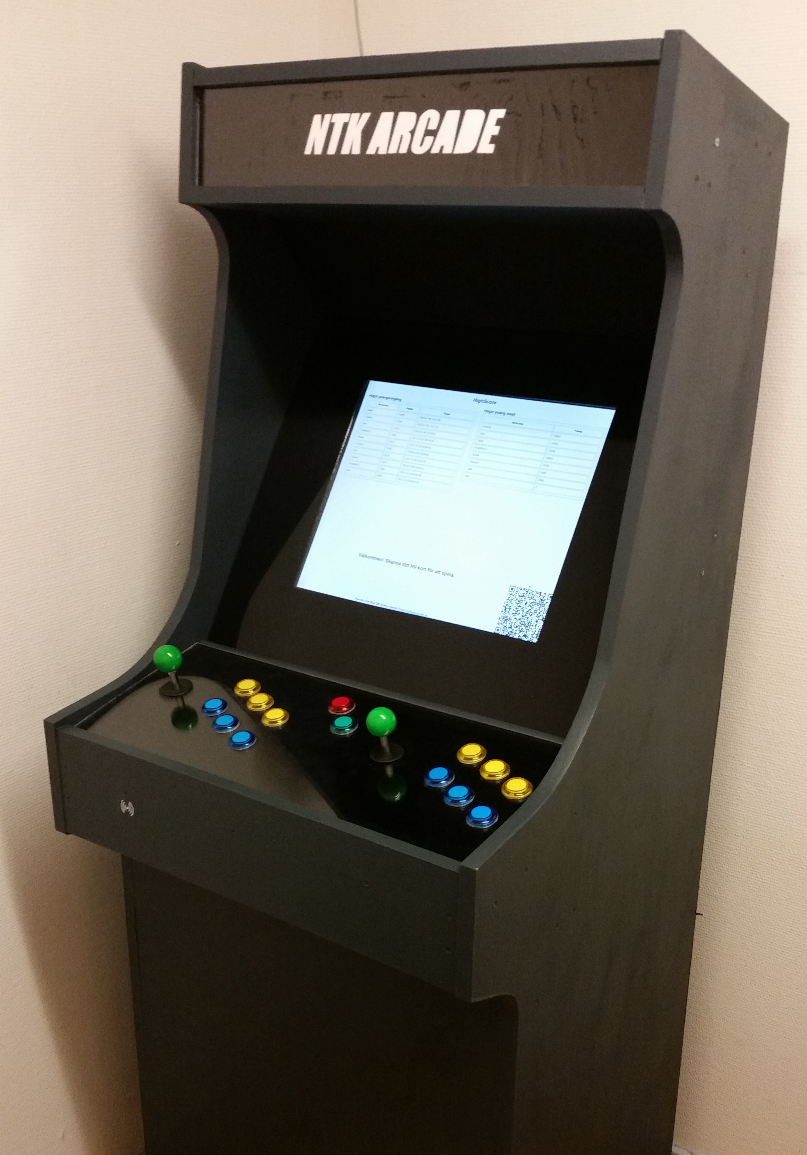
\includegraphics[width=\paperwidth]{cabinet}};
\draw (current page.center) node [fill=black,fill opacity=0.8,text opacity=1,text=white,inner sep=1cm]{\Huge\centering\bfseries\sffamily\parbox[c][][t]{\paperwidth}{\centering Arkadprojekt\\[15pt] % Book title
{\Large med RFID avläsning}\\[20pt] % Subtitle
{\normalsize Simon Olofsson, Olof Ivarsson, Madeleine Karlsson, Patrick Lundin, Sara Andersson, Emrik Olsson}}}; % Author name
\end{tikzpicture}
\vfill
\endgroup

%----------------------------------------------------------------------------------------
%	COPYRIGHT PAGE
%----------------------------------------------------------------------------------------

\newpage
~\vfill
\thispagestyle{empty}

\noindent Revision history: v1.0 - Mon, Jan 8 2018.

%\noindent Copyright \copyright\ 2013 John Smith\\ % Copyright notice

%\noindent \textsc{Published by Publisher}\\ % Publisher

%\noindent \textsc{book-website.com}\\ % URL

%\noindent Licensed under the Creative Commons Attribution-NonCommercial 3.0 Unported License (the ``License''). You may not use this file except in compliance with the License. You may obtain a copy of the License at \url{http://creativecommons.org/licenses/by-nc/3.0}. Unless required by applicable law or agreed to in writing, software distributed under the License is distributed on an \textsc{``as is'' basis, without warranties or conditions of any kind}, either express or implied. See the License for the specific language governing permissions and limitations under the License.\\ % License information

%\noindent \textit{First printing, March 2013} % Printing/edition date

%\noindent \textit{(This page left intentionally blank)}

%----------------------------------------------------------------------------------------
%	TABLE OF CONTENTS
%----------------------------------------------------------------------------------------

%\usechapterimagefalse % If you don't want to include a chapter image, use this to toggle images off - it can be enabled later with \usechapterimagetrue

\chapterimage{chapter_head_tyrian_logo.pdf} % Table of contents heading image

\pagestyle{empty} % No headers

\tableofcontents % Print the table of contents itself

% \cleardoublepage % Forces the first chapter to start on an odd page so it's on the right

\pagestyle{fancy} % Print headers again

%----------------------------------------------------------------------------------------
%	PART
%----------------------------------------------------------------------------------------

%\part{Part One}

%----------------------------------------------------------------------------------------
%	CHAPTER 1
%----------------------------------------------------------------------------------------

\chapterimage{tyrian_header.jpg} % Chapter heading image

\chapter{Introduktion}

\section{Bakgrund}\index{Bakgrund}
Vi påbörjade en kurs som heter Praktisk datateknik där vi fick möjlighet att själva välja vilket projektarbete vi ville göra. Vår grupp
bestod av sex personer som enades om att bygga en arkadmaskin. Idén var att bygga en arkadmaskin där studenter på högskolan kunde spela 
på ett enkelt sätt genom att använda sina Högskolan Väst-kort. Dessa kort används bland annat för att komma in och ut genom dörrar i 
byggnaderna och låna böcker. För att kunna genomföra idén med betalning med studenternas kort krävdes det att kortläsaren kunde läsa 
RFID-chippet på samma frekvens som korten är inställda på och även kunna skicka information till en extern server.

På den externa servern skulle hantering av spelarprofiler, registrering av användare och kredithanteringen skötas för att kunna spela på arkadmaskinen
samt att skicka information som att spelet skall öppnas på arkaden när det finns tillräckligt med krediter hos spelaren. Ett annat mål 
var att om en spelare inte var registrerad eller hade krediter för att kunna spela skulle det visas en QR-kod som kan skannas och som 
tar spelaren till hemsidans registreringssida alternativt till profilsidan för att fylla på krediter om man redan är registrerad. 

Projektet behövde ta ställning till vilken typ av spel som kunde användas. Då vi hade planerat att använda en kortläsare för att kunna 
ta betalt av potentiella spelare kom vi fram till att det fick bli ett open-source spel. Detta gjorde att vi inte behövde ta hänsyn till
olika spelrättigheter. Spelet som valdes heter Tyrian och blev tillgängligt som freeware 2004. Spelaren styr ett rymdskepp utrustat med 
olika skjutvapen och ska skjuta fiender och samla poäng och power-ups i sann arkad anda.

Till en början funderade vi på att designa arkadmaskinen med litet kabinett som skulle stå på ett bord för att komma upp i högre höjd
men vi kom snabbt fram till att vi ville göra en i full storlek, ca 170 cm högt. Det material som valdes var 19 mm MDF skiva, plexiglas
samt regel och detta har Karl Hedin i Vänersborg sponsrat oss med. En fundering/ett problem vi hade var hur vi skulle såga ut alla delar
perfekt utifrån vår CAD ritning då ingen av oss hade tillgång till de verktyg eller utrymme som krävdes. Detta löstes genom att Magnus
Åbergsgymnasiets (MÅG) byggprogram tillfrågades och genom deras kompetens fick vi delarna precis så som vi ville ha dem.

\section{Systembeskrivning}\index{Systembeskrivning}
%\subsection{Användning och arkitektur}\index{system!Användning}
%\subsection{Användning}\index{system!Användning}
Användaren börjar med att skanna sitt Högskolan Väst-kort på framsidan av arkadmaskinen. Första gången kortet skannas så visas ett 
meddelande om att registrering krävs innan man får spela och en QR-kod presenteras. Genom att skanna koden med sin smartphone öppnas 
hemsidan arkadprojekt.se som är kopplad till projektet. Där skapar man sitt konto och kan sedan ladda på krediter på sin profilsida. 
När kortet skannas på arkadmaskinen nästa gång startas spelet Tyrian. Spelet fortgår tills game over eller om krediterna tar slut. 
Då avslutas spelet och startsidan på arkadmaskinen visas igen. Om spelaren saknar krediter på kontot visas information om detta och 
genom att gå in på sin spelarprofil är det enkelt att fylla på mer. Därefter går det att spela igen.
\bigskip

%\subsection{Arkitektur}\index{system!Arkitektur}
Arkadmaskinen består av flera entiteter som tillsammans skapar arkadsystemet. Den fysiska vyn i Figur \ref{fig_physview} visar informationsflödet 
mellan dessa entiteter. Datorn Raspberry Pi kör kontinuerligt ett pythonscript som läser data från Högskolan Väst-kortet via kortläsaren. 
När kort-ID är inläst kommunicerar datorn med ett webAPI för att kontrollera huruvida kortet finns registrerat i systemet eller ej. För 
icke-registrerade kort genereras en QR-kod för användaren som leder till hemsidan som ligger på webbservern. Där kan användaren 
registrera sig och ladda på krediter. Nu finns användarinformation och kopplat kort-ID lagrat i databasen. För registrerade kort med 
krediter körs spelet och datorn tolkar signaler från knappar och joystick. Gränssnittet mellan användare och arkadmaskin är skärmen 
och högtalarna.

\begin{figure}[!h]
\centering\fbox{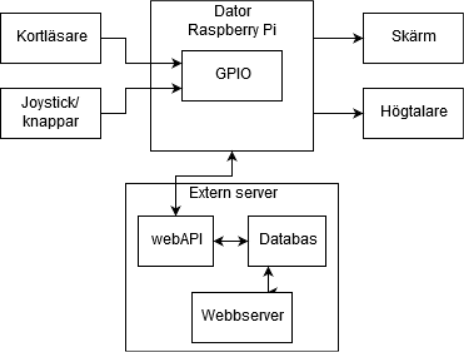
\includegraphics[width=.5\textwidth]{physicalview}}
\caption{Fysisk vy över Arkadmaskinens entiteter}
\label{fig_physview}
\end{figure}

%----------------------------------------------------------------------------------------
%	CHAPTER 2
%----------------------------------------------------------------------------------------

\chapterimage{headercode.png}
\chapter{Design och implementering}
\section{Chassi}\index{design!Chassi}
Gruppen diskuterade till en början att göra ett litet kabinett som skulle behöva stå på ett högre bord om man vill stå upp och
spela men vi kom snabbt fram till att göra ett i full storlek på 170 cm. Funderingen kring utsågning av material löstes av elever
på Magnus Åbergsgymnasiets (MÅG) byggprogram för att få dem enligt vår CAD ritning. Design och mått gjordes i Autodesk Inventor 
2018 med grund-design taget från koenigs.dk\footnote{http://www.koenigs.dk/mame/eng}.

Det som användes var två stycken MDF skivor, två plexiglas, en regel till bottenplatta samt att stödja upp nederdelen av skåpet. 
Detta har sponsrats av Karl Hedin i Vänersborg. Invändigt för att montera fast de MDF skivor som användes till högtalare, tak, 
frontpanel, kontrollbräda och den liggande brädan under kontrollbrädan användes planhyvlat virke. Kvartsstaven användes för att 
skapa en snyggare övergång mellan skärmen och kontrollbrädans kanter. Tabell \ref{table_material} listar allt material och Figur \ref{fig_material} är de utsågade delarna.

\begin{table}[h]
\centering\resizebox{.9\textwidth}{!}{%
\begin{tabular}{ ||c|c|c|| } 
 \hline
 Chassi & Hårdvara & Övrigt \\ [0.5ex]
 \hline\hline
 2st MDF 19x1200x2400 mm & Raspberry Pi & Färg + penslar \\ 
 1st Regel 45x95x2700 mm & Arkadknappar 14st & Designfolie \\ 
 2 st Plexiglas 3x600x750 mm & Joystick 2 st & Tyg till högtalarbrädan \\
 1 st Kvartsstav 9x9x900 mm & Skärm & Belysning \\
 Hjul & Högtalare & Diverse lämpliga verktyg \\
 Dörrhängare & Kablar & \\
 Lås & Hålband till högtalarna & \\
 Skruv & Flatstifthylsor & \\
 Handtag & & \\
 \hline
\end{tabular}}
\caption{Material som användes}
\label{table_material}
\end{table}

\begin{wrapfigure}[17]{R}{0.35\textwidth}
  \begin{center}
    \fbox{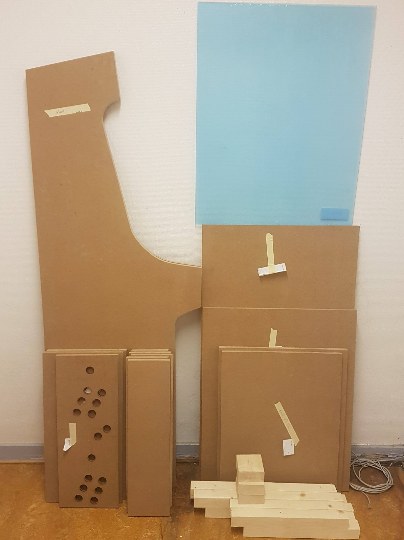
\includegraphics[width=0.3\textwidth]{materialdelar}}
  \end{center}
  \caption{Det utsågade materialet}
  \label{fig_material}
\end{wrapfigure}
\newpage
Det som var viktigt att tänka på under hela monteringen av chassit var att nästa steg fick övervägas innan delarna sattes fast 
för att inte göra det svårare i nästa moment. För att dölja insidan av skåpet och ramen på skärmen användes designfolie på framsidan 
av plexiglaset. Skärmens kanter målades svarta med nagellack för att de inte skulle synas från sidan. Brädan för högtalarna har två
utsågade hål och högtalarna sitter fastspända på baksidan med hålband. För att dölja de utsågade hålen som gjorts är ett tyg fastspänt
över. Vi valde senare att designa kontrollbrädan med plexiglas. Detta medförde att de redan utsågade hålen i MDF skivan var för små 
och detta löstes genom att fräsa ur dem lite. Det behövdes även fräsas för att joystickarna skulle komma upp mer. Hålen i plexiglaset
ritades ut med hjälp av ursprungsbrädan och en hålsåg användes för att göra hålen. För att dölja MDF materialet användes även här 
designfolie och hålen skars ut men inte hela vägen runt utan i snitt in mot mitten. Vi hittade ingen bra bild att använda till bannern 
så beslutet blev att skära ut “NTK ARCADE” i designfolie och sätta mellan de två plexiglasen.

\section{Hårdvara och mjukvara}\index{design!Dator och kortläsare}
\subsection{Dator och kortläsare}\index{design!Översikt}
Enkortsdatorn Raspberry Pi 3 valdes som hårdvaruplattform i projektet. Den främsta anledningen är att datorn erbjuder flertalet
externa anslutningsmöjligheter, vilket var en förutsättning för att kunna koppla in kortläsare, knappar och joystick, se Figur \ref{fig_knappar}. Datorn 
erbjuder också god prestanda för enklare 2D- och 3D-applikationer samt att energiförbrukningen är låg. Kortläsaren i projektet 
bestod av en RFID-läsare med kretsen RC-522, se Figur \ref{fig_pirfid}. Valet baserades på att kretsen skulle stödja Högskolan Väst-korten, som är av typen 
MIFARE och använder 13,56MHz frekvens för kommunikation. Det var också viktigt att kortläsaren var kompatibel med datorn i termer 
av drivrutinsstöd och fysisk anslutning.

\begin{figure}[!htb]
  \begin{minipage}{0.44\textwidth}
    \centering
    \fbox{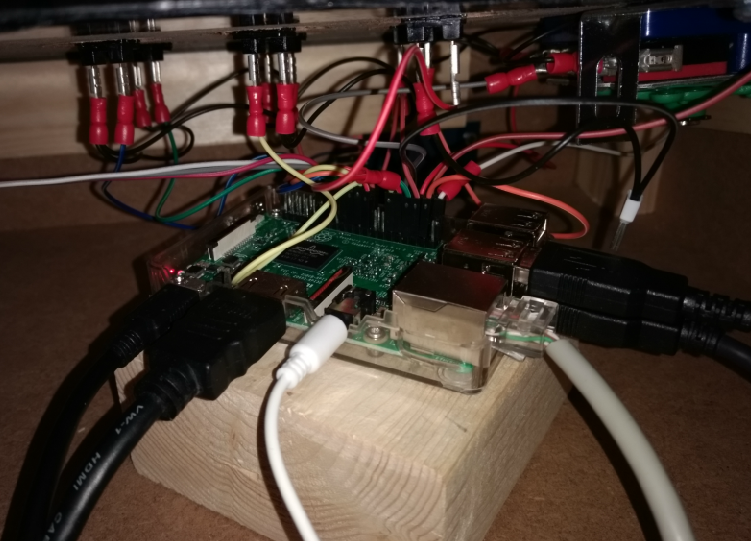
\includegraphics[width=.9\linewidth]{rpi-arkad}}		
    \caption{Knappar och joystick inkopplade}
    \label{fig_knappar}
  \end{minipage}\hfill
  \begin{minipage}{0.44\textwidth}
    \centering
    \fbox{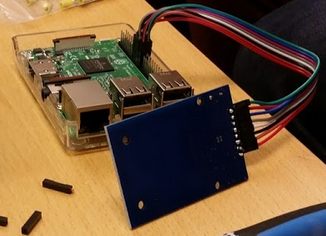
\includegraphics[width=.9\linewidth]{piwithrfid}}
    \caption{Raspberry PI med kortläsare (RC-522)}
    \label{fig_pirfid}
  \end{minipage}\hfill 
\end{figure}

%\subsection{Inkoppling}\index{design!Inkoppling}
Kortläsaren kopplas till datorn via en Serial Peripheral Interface (SPI) port. Den synkrona seriella kommunikationen styrs av 
datorn som agerar masterenhet. Kortläsaren drivs via datorns inbyggda 3,3V-matning. För att läsa data från Högskolan Väst-korten 
installerades drivrutiner för kortläsaren samt modulen SPI-Py. Modulen inkluderar bibliotek med färdiga funktioner för att enklare 
kunna kommunicera via SPI-porten. Knappar och Joystick ansluts till godtyckliga General Purpose Input Output (GPIO) portar på datorn 
och mappas till spelet Tyrian via mjukvara. Se Figur \ref{fig_gpio} för inkopplings-schema.

\begin{figure}[h]
\centering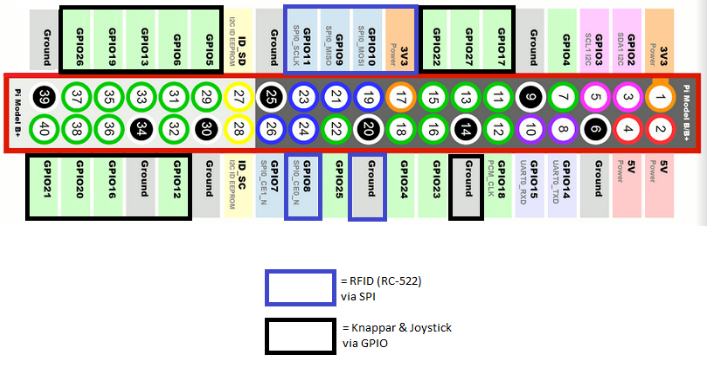
\includegraphics[width=.8\textwidth]{gpio}
\caption{Använt kopplingsschema för kortläsaren och arkad input}
\label{fig_gpio}
\end{figure}

\subsection{Arkadens Mainloop}\index{design!Mainloop}
Programmet som körs på arkadmaskinen är skrivet i Python och styr kopplingen mellan skanningen av RFID-kort och startande av spel. 
Efter att spelaren har spelat klart sparas även information om spelsessionen såsom hur mycket poäng spelaren fick och speltid. 
Den informationen presenteras sedan på hemsidan som en highscore-lista. I Figur \ref{fig_mainloop} visas med pseudo-kod hur programmet är uppbyggt. 

\begin{figure}[!h]
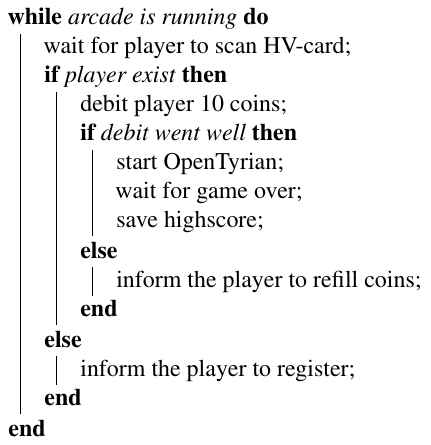
\includegraphics[width=.4\textwidth]{mainloop}
\label{fig_mainloop}
\caption{mainloop körandes på arkadmaskinen}
\end{figure}

\subsection{Modifiering av OpenTyrian}\index{design!OpenTyrian}
För att få spelet att fungera som vi ville fullt ut behövdes viss modifikation göras. En av ändringarna som gjordes 
gäller spelmenyn som visas mellan de olika episoderna i spelet. I den menyn skulle användaren kunna ändra options för 
spelet samt kunna gå tillbaka till huvudmenyn och göra ytterligare ändringar. 
För att förhindra detta gjordes ändringar i koden enligt Figur \ref{fig_opentyrian} där valet för options i menyn 
(“case 3” i koden) kommenterats bort helt samt att om spelaren väljer quit i menyn (“case 4” i koden) så skapas en 
fil med namn QUIT\_GAME\_TRUE som pythonskriptet kontinuerligt kontrollerar om den finns. När pythonskriptet upptäcker 
filen stängs spelet av helt istället för att spelaren skulle komma tillbaka till spelets huvudmeny.

\begin{figure}[!h]
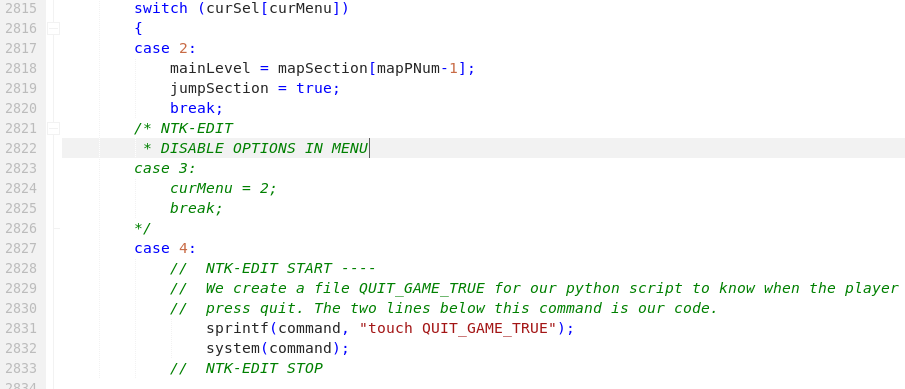
\includegraphics[width=\textwidth]{opentyrian}
\caption{Ändring av game\_menu.c för att inaktivera options-menyn och skapa fil vid avslut}
\label{fig_opentyrian}
\end{figure}
Exempel på andra ändringar som gjorts var även att spara highscore till en fil som pythonskriptet kan läsa av vid 
spelets slut samt inaktivera huvudmenyn vid spelets start så spelaren kommer in i ett spel direkt utan att behöva 
trycka i menyn.

\begin{wrapfigure}{r}{0.45\textwidth}
  \begin{center}
    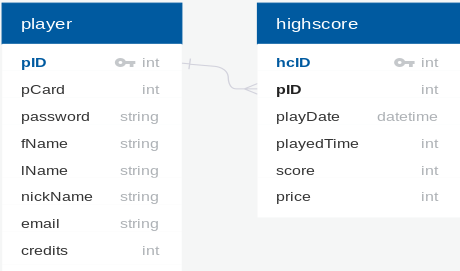
\includegraphics[width=0.4\textwidth]{databas}
  \end{center}
  \caption{Databastabeller}
  \label{fig_databas}
\end{wrapfigure}

\section{Server}\index{design!Server}
\subsection{Databas}\index{design!Databas}

Databasen som används är MariaDB\footnote{[https://mariadb.org/about/}. Kommunikationen mellan arkadmaskinen och databasen 
sker via ett webAPI skrivet i PHP. På detta sätt blir systemet skalbart och ändringar kan lätt göras utan att behöva göra 
ändringar direkt på arkadmaskinen. Databasen är uppbyggd av två tabeller: player och highscore, se Figur \ref{fig_databas}.
\clearpage
I player sparas information om spelare såsom namn, epost med mera. I highscore sparas information efter varje spelrunda som
har gjorts med hur mycket poäng spelaren fick, hur länge spelet pågick med mera. Nedan i tabell \ref{table_databas} förklaras de olika fälten
i tabellerna mer noggrant.

%\clearpage\newpage

\begin{table}[!h]
\centering
\resizebox{\textwidth}{!}{%
\begin{tabular}{ ||l|l|l|l|| } 
 \hline
 \multicolumn{2}{||c|}{Player} & \multicolumn{2}{|c||}{Highscore}  \\
 \hline
 Fält & Förklaring & Fält & Förklaring \\
 \hline\hline
 pID & spelarens ID & hcID & highscore ID \\
 pCard & spelarens kortnummer (HV-kort) & pID & spelarens ID \\
 password & lösenord & playDate & datum för spelsessionen \\
 fName & förnamn & playedTime & antal sekunder spelsessionen varade \\
 lName & efternamn & score & antal poäng spelaren fick \\
 nickName & spelarnamn & price & hur många coins spelrundan kostade \\
 email & epost & & \\
 credits & antal coins & & \\
 \hline\hline
\end{tabular}}
\caption{Förklaring av databastabell}
\label{table_databas}
\end{table}

\subsection{Hemsida}\index{design!Hemsida}

Vi köpte domännamnet arkadprojekt.se som hålls av Binero och för att bygga upp hemsidans design och funtioner användes HTML, CSS och PHP.

De funktioner som framförallt behövs på hemsidan är möjligheten som spelare att kunna logga in och fylla på coins för att sedan kunna spela 
på arkadmaskinen. Utöver denna funktion har vi med highscore hämtat från spelet, information om oss som grupp, information om arkadmaskinens 
historia samt om spelet Tyrian. Vi valde även att ha med en supportsida där man kan ta kontakt med någon av gruppmedlemmarna via mail om det 
skulle vara något med maskinen eller spelet som inte skulle fungera. Hemsidan är utformad med de mest nödvändiga funktionerna och hålls väldigt stilren, se Figur \ref{fig_hemsida}
\begin{figure}[h]
\centering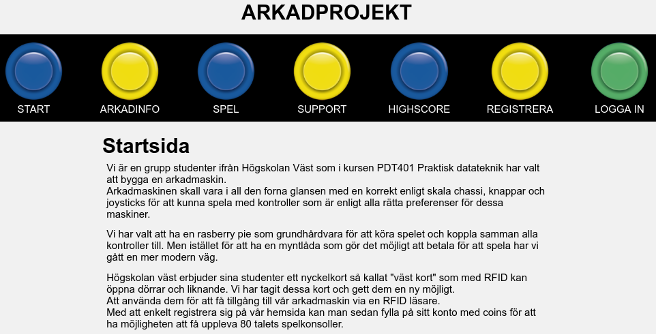
\includegraphics[width=\textwidth]{hemsida}
\caption{Projektets hemsida}
\label{fig_hemsida}
\end{figure}

%----------------------------------------------------------------------------------------
%	CHAPTER 3
%----------------------------------------------------------------------------------------
\chapterimage{analys.jpg}
\chapter{Designanalys}


\section{Chassi}\index{analys!Chassi}
Valet att bygga ett större kabinett grundades i att vi förmodligen bara skulle göra detta en gång och att vi ville göra det 
rejält och så likt de klassiska arkadmaskinerna som möjligt. När det kommer till utsågning av material och att det blev elever 
på MÅG som gjorde det var för att ingen i gruppen har större erfarenhet kring detta och vi ville ha delarna så perfekta det 
bara gick. Att det blev MDF som material grundades i att de flesta ritningar och guider använde MDF och det var det bästa 
alternativet. Att vi gjorde valet med att sätta plexiglas på kontrollbrädan var för att det gav ett mer autentiskt intryck, se Figur \ref{fig_kontrollpanel}. 

\begin{figure}[h]
\centering\fbox{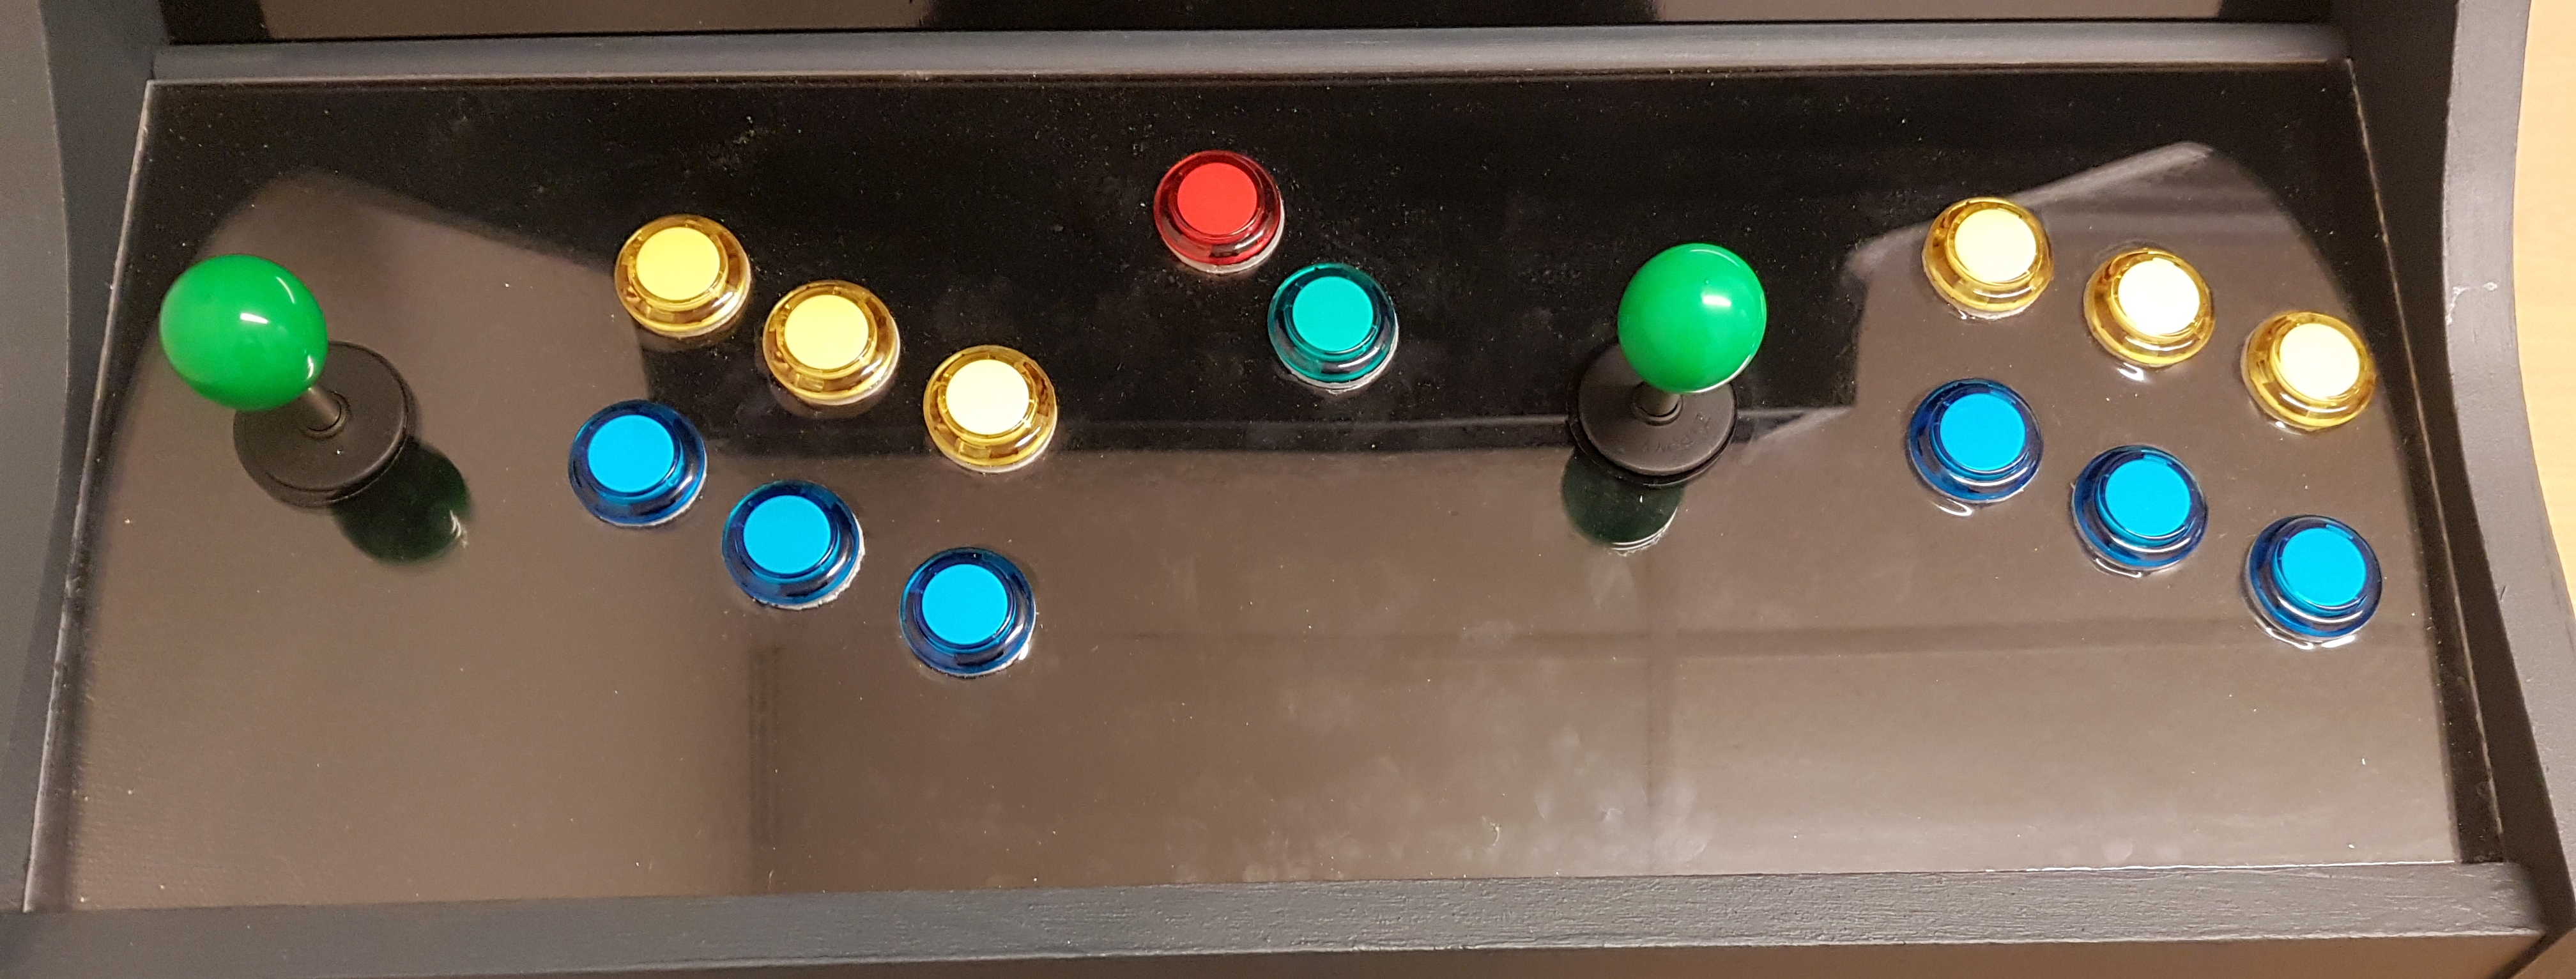
\includegraphics[width=.6\textwidth]{kontrollpanel}}
\caption{Kontrollpanelen}
\label{fig_kontrollpanel}
\end{figure}

\section{Dator och kortläsare}\index{analys!Dator och RFID-läsare}
%\begin{wrapfigure}[13]{r}{0.25\textwidth}
%  \begin{center}
%    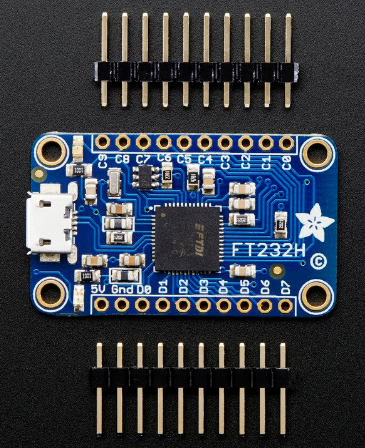
\includegraphics[width=0.2\textwidth]{breakout}
%  \end{center}
%  \caption{Breakout board}
%  \label{fig_breakout}
%\end{wrapfigure}
Enkortsdatorn Raspberry Pi 3 har flera positiva egenskaper som ligger till grund för projektets val av dator:

\begin{itemize}
 \item Liten
 \item Billig
 \item Flera anslutningsmöjligheter
 \item Energisnål
 \item God prestanda för enklare applikationer och spel
 \item Stort utbud i butik
\end{itemize}
\bigskip

Det finns dock andra dator- och anslutningsalternativ som kan ha fungerat lika bra. Arkadmaskinens chassi har exempelvis gott med utrymme 
för att kunna använda en traditionell och mer kraftfull dator. Detta vore nödvändigt för mer krävande system. För att lösa utmaningen med 
inkoppling av kortläsare, knappar och joystick så finns det s.k breakout boards som en lösning. Dessa boards kan tillhandahålla anslutningar 
såsom RS232, SPI, I2C, realtidsklocka och vanlig GPIO. Ofta kommunicerar dessa kort med datorn via USB. Valet av kortläsaren baseras på att 
den är kompatibel med Högskolan Väst-korten, är kompatibel med datorn och att den fanns tillgänglig att köpa i butik. Hade projektet använt 
en traditionell dator utan stöd för SPI så finns det andra kortläsare som kommunicerar seriellt via RS232. Alternativt använder man en 
breakout board med rätt anslutningar.

\section{Server}\index{analys!Server}

\subsection{Hemsida}\index{analys!Hemsida}

Vi valde att ha med flera olika underrubriker än de rent användbara som “logga in” och “registrera”, se Figur \ref{fig_profilsida}.
Detta då vi ansåg att det blev väldigt tomt utan, och utfyllnaden gav hemsidan en bättre känsla av att vara komplett med information om 
oss, om arkadmaskiner generellt samt om spelet som vi hade med. Hemsidan med sitt stilrena utseende fick i navigeringsfältet ta med inspiration av arkadmaskinen genom att navigeringsknapparna blev 
omvandlade till arkadknappar. 

\begin{figure}[h]
\centering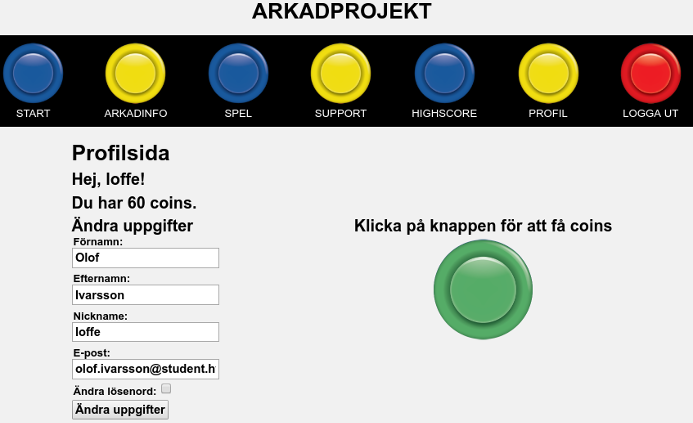
\includegraphics[width=.9\textwidth]{profil}
\caption{Inloggad på hemsidan, profilsidan}
\label{fig_profilsida}
\end{figure}

En sak som ansågs vara viktigt, att kunna se highscore på hemsidan, se Figur \ref{fig_highscore}. Detta för att inspirera våra spelare att förbättra sig och kunna
jämföra nya resultat mot deras äldre, samt att ha något att sträva efter i form av att ligga på första plats.

\begin{figure}[!h]
\centering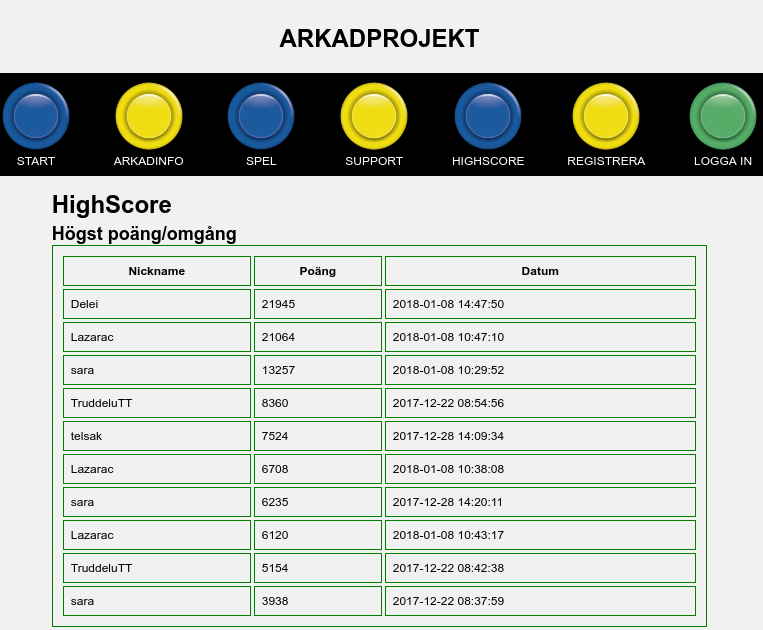
\includegraphics[width=.9\textwidth]{highscore}
\caption{Highscore lista på hemsidan}
\label{fig_highscore}
\end{figure}

Vi valde att köpa domännamnet arkadprojekt.se då vi hittade detta till ett billigt pris, ett väl passande namn. Hade vi inte hittat
detta så var tanken att vi skulle använda oss av ett gratis domännamn som inte hade givit oss ett lika passande namn, samt att vi inte
hade fått lika stor frihet i namnet som i den köpta utvalda domänen.  

Anledningen till att PHP användes var för att vi använder oss av operativsystemet Linux på servern och då kändes detta som det mest 
naturliga alternativet. Detta även för att det i gruppen fanns kunskaper sedan tidigare om användandet av PHP.

%----------------------------------------------------------------------------------------
%	CHAPTER 4
%----------------------------------------------------------------------------------------
\chapterimage{gruppen.png} % Chapter heading image
\chapter{Projektreflektioner}


Gruppens reflektioner kring arbetet är att vi som grupp haft en god kontakt sinsemellan med avstämningsmöten en gång i veckan, nära 
arbete och en messenger konversation som användes i form av intern kommunikation för gruppen.

Då vi var 6 personer delade vi upp arbetet enligt dess natur (hårdvara, mjukvara, hemsida etc) och delade därefter upp ansvarsområdet 
på oss i mindre grupper. På så sätt fick vi alla ett bestämt ansvarsområde medan man fanns tillgänglig för att ge stöd åt en annan 
grupp om det behövdes. Våra möten blev mer avstämningar för att kontrollera och rapportera statusen för de diverse ansvarsområdena 
samt ett sätt att se till att viktig information eller dylikt kom ut utan att det sägs snabbt i korridoren och därmed lätt missas 
eller glöms av. Som helhet har projektet gått bra. Vi har löst uppkomna problem under arbetets gång och fått ut en fullt fungerade arkadmaskin. 

\end{document}